\part{Vehicle Routing Problem}
车辆路径规划问题(Vehicle Routing Problem, VRP\index{VRP})是物流配送领域中的核心优化问题之一,由George Dantzig和John Ramser于1959年首次提出\cite{1959The}。其目的是为一组具有容量限制的车辆设计最优配送路线,使得所有客户需求被满足且总运输成本(如距离、时间或费用)最小化。当车辆容量足够大时,VRP退化为TSP,即当车辆容量足够时,所有货物都可以在一次行驶中全部配送,只需要经过一次配送中心。大多数情况下VRP的车辆容量总是小于需要配送的所有货物重量的总和,所以与旅行商问题(TSP)不同,VRP需要同时考虑多车辆协同、客户需求分配、车辆容量限制等复杂约束,因此更具现实意义和研究挑战性。

\begin{figure}[!htb]
    \centering
    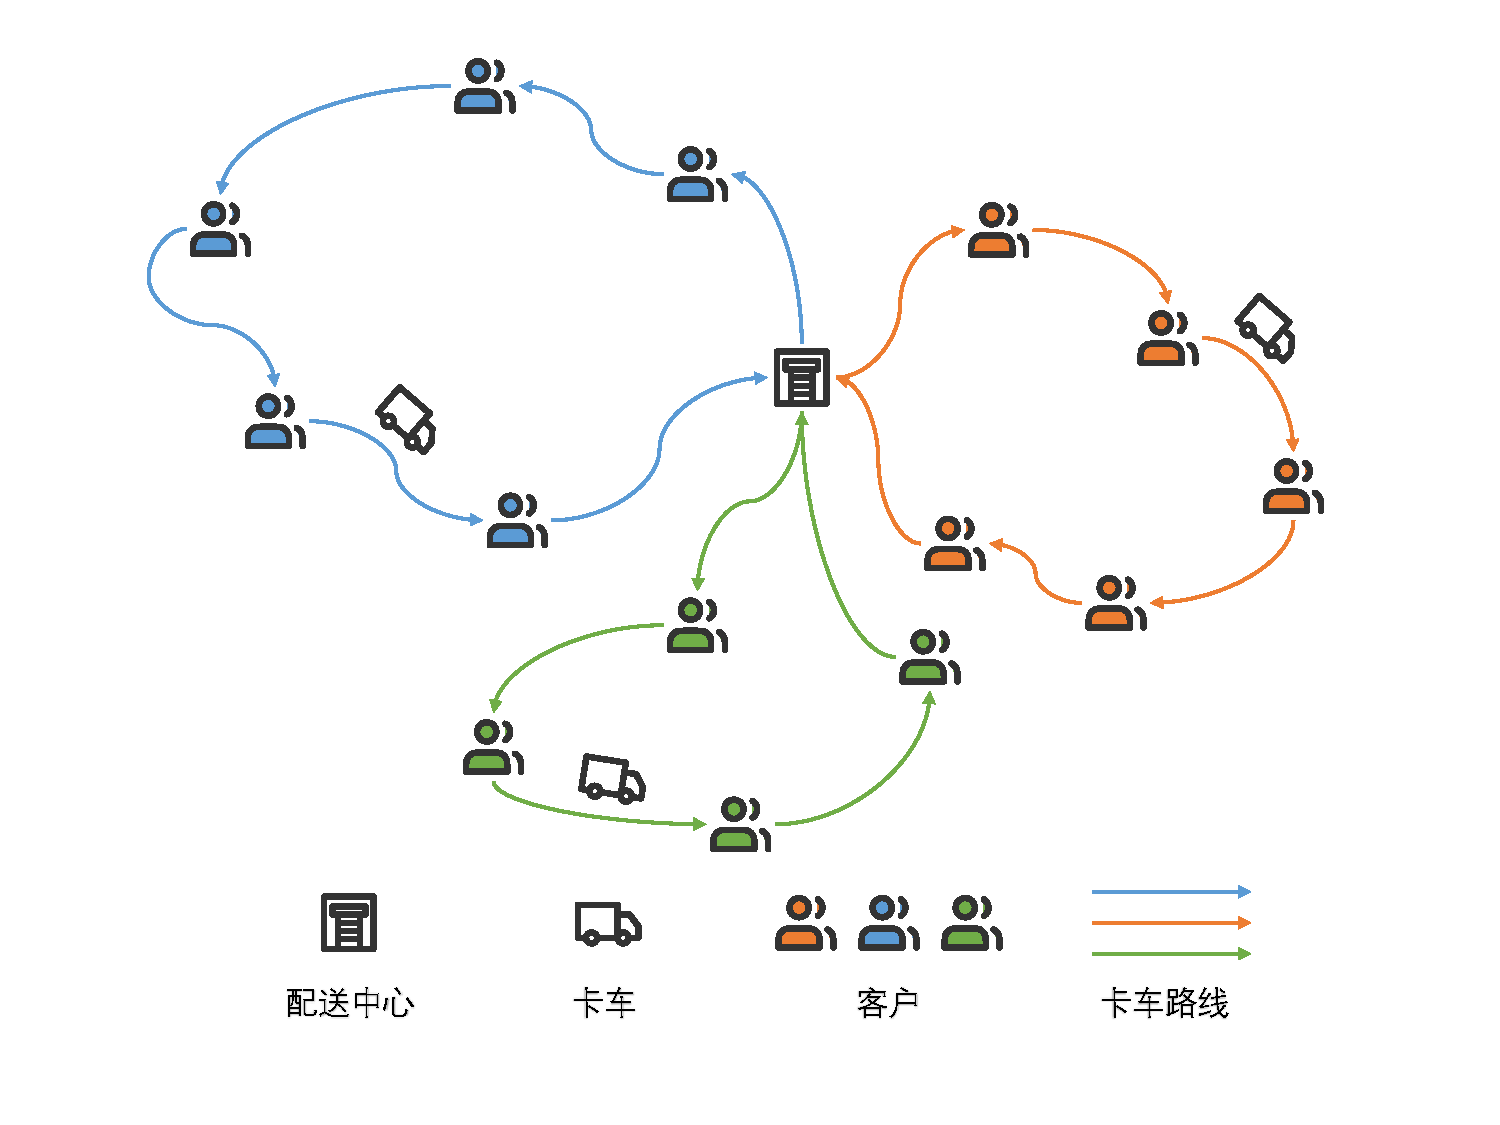
\includegraphics[width=\linewidth]{images/VRP.pdf}\\
    \caption{VRP示意图}
\end{figure}

VRP可以表述为整数规划问题\cite{2014Vehicle}:假设存在一个配送中心(仓库)和若干顾客点,顾客点需求为$q_i(i = 1,2,\cdots,n)$,车辆载重上限为$Q$,每辆车从仓库出发并最终返回仓库。定义决策变量$x_{ijk} = \begin{cases}1, & \text{车辆$k$从$i$行驶到$j$}\\0, & \text{其他} \end{cases}$,节点集合$V = \{0, 1, 2, \cdots, n\}$,其中0表示配送中心,$S = \{1,2,\cdots,n\}$表示顾客节点,车辆集合$K = \{1,2,\cdots,m\}$,$c_{ij}$表示从点$i$到点$j$的行驶成本(距离或时间),同样在VRP中为了消除子回路,引入辅助变量$u_i$表示车辆访问顾客点$i$时的累计载重量。因此,VRP的数学模型可以表示为MILP \ref{model:model-vrp}。

\begin{model}{MILP VRP}{model-vrp}
\begin{align}
    \min \quad & \sum_{k \in K}\sum_{i \in V}\sum_{j \in V, j \neq i} c_{ij}x_{ijk} & \label{eq:vrp-obj}\\
    \text{s.t.} \quad & \sum_{j \in S} x_{0jk} = 1, & \forall k \in K\label{eq:vrp-in}\\
    \quad & \sum_{i \in S} x_{i0k} = 1, & \forall k \in K\label{eq:vrp-out}\\
    \quad & \sum_{k \in K}\sum_{i \in V, i \neq j} x_{ijk} = 1, & \forall j \in S\label{eq:vrp-customer}\\
    \quad & \sum_{i \in V, i \neq j}x_{ijk} = \sum_{i \in V, i \neq j} x_{jik}, & \forall j \in V, k \in K\label{eq:vrp-flow}\\
    \quad & u_j \geq u_i + q_j -Q(1 - x_{ijk}), & \forall i, j \in S, k \in K\label{eq:vrp-subtour}\\
    \quad & q_j \leq u_j \leq Q, & \forall j \in S\label{eq:vrp-subtour2}\\
    \quad & x_{ijk} \in \{0, 1\}, & \forall i, j \in V, k \in K\label{eq:vrp-x_bound}
\end{align}
\end{model}

目标函数\ref{eq:vrp-obj}表示最小化所有车辆的总行驶成本,约束\ref{eq:vrp-in}和\ref{eq:vrp-out}确保每辆车从配送中心出发并最终返回,约束\ref{eq:vrp-customer}保证每个顾客点只被访问一次,约束\ref{eq:vrp-flow}保证了流量守恒,即保证了路径的连续性,约束\ref{eq:vrp-subtour}和\ref{eq:vrp-subtour2}通过MTZ方法消除子回路并满足车辆的容量限制,约束\ref{eq:vrp-x_bound}对变量进行限制。
